% Nome do capítulo
\chapter{METODOLOGIA}
% Label para referenciar
\label{cap3}

% Diminuir espaçamento entre título e texto
\vspace{-1.9cm}

% Texto do capítulo

    Para que o desenvolvimento do trabalho esteja alinhado as necessidades do laboratório de audiovisual e fotografia seria preciso, em um primeiro momento, elicitar todos os requisitos arquiteturais (funcionais e não funcionais) de maneira que o entedimento do escopo do projeto fique claro. Os requisitos são descritos textualmente para identificar as funcionalidades e características que a aplicação deve possuir para conseguir realizar as ações que, em conjunto, solucionam o problema exposto, sendo assim, tem-se uma visão de alto nível do projeto, o que torna sua interpretação fácil a todos os envolvidos.
    
    Com a definição do escopo do projeto e dos requisitos, seria criado um protótipo da parte visual que contemple as principais interfaces do aplicativo e seus respectivos componentes, além de elaborar diagramas de classe e de componentes que retratam como o software irá se comportar de maneira oculta e como esses componentes irão persistir dados, a estrutura lógica do banco de dados e qual tipologia de dados seria mais adequeada ao problema que este trabalho irá resolver. Dado a criação destes diagramas que apresentam a arquitetura de funcionamento do software é possível compreender como será o fluxo de comunicação do aplicativo e a apresentação das informações pertinentes aos usuários durante o uso.
    
    Conforme apresentado na figura \ref{figura:lab-architecture} é possível visualizar a arquitetura da aplicação \textit{mobile}, o fluxo de comunicação entre os componentes e os padrões de projeto adotados para desenvolver esta solução, na API Rest desenvolvida para suportar as funcionalidades do aplicativo e suas operações no banco de dados, encontra se o padrão MVC, semelhante ao padrão MVP, apresentado na subseção \ref{react_native_mvp} e que foi aplicado no aplicativo em \textit{React Native}.
    
    \clearpage
    
    \begin{figure}[h]
    \caption{Arquitetura do aplicativo}
    \centering % para centralizarmos a figura
    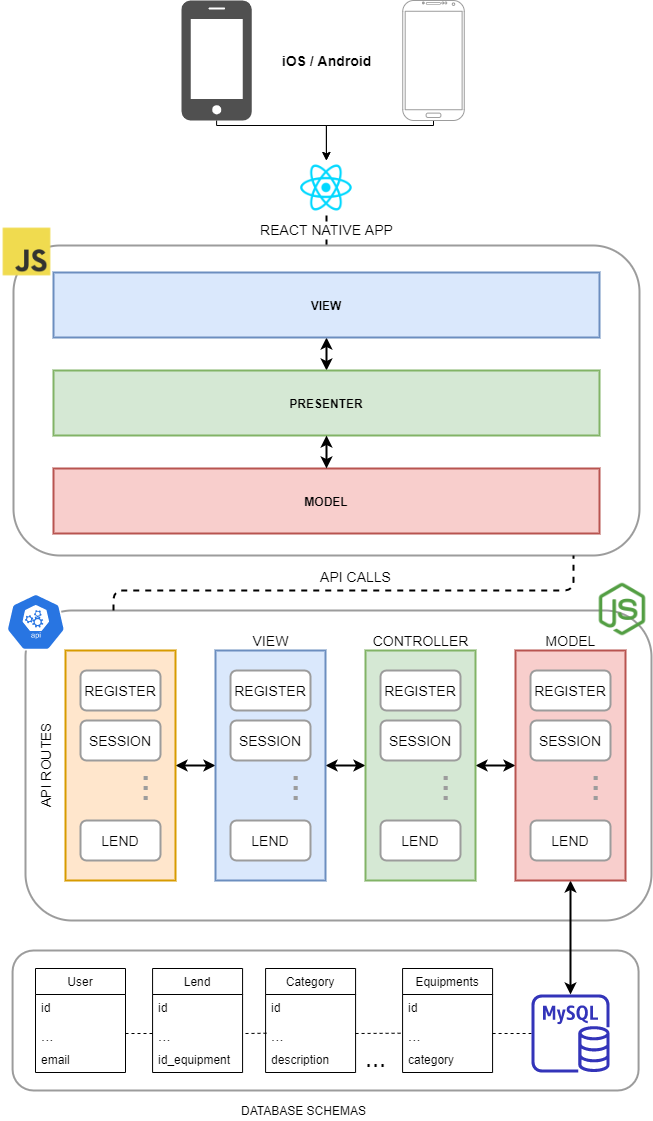
\includegraphics[width=12cm]{imagem/jubilant-octo-lab.png}
    \caption*{Fonte: Autor}
    \label{figura:lab-architecture}
    \end{figure}
    
    \clearpage
    
    Após essas definições de arquitetura, citadas no paragráfo anterior, serão selecionadas as ferramentas e as principais bibliotecas disponibilizadas pelo JavaScript para compor o processo de desenvolvimento e a codificação do aplicativo, junto à escolha da estrutura de hierárquica de diretórios, configuração do ambiente de desenvolvimento e ambiente para os testes.
    
    A penúltima etapa consiste no desenvolvimento do aplicativo em si, considerando todos requisitos pré definidos e seguindo as especificações de interface elaborada na etapa de prototipagem e a escrita dos testes unitários e de integração para validar o comportamento do sistema perante o uso de suas funcionalidades, simulando objetos/usuários reais com metódos disponibilizados pelas bibliotecas que estão em uso na aplicação.
    
    E por fim, a implantação e disponibilização do aplicativo em Android e iOS, para alguns alunos e monitores da Universidade para analisar como o sistema se comporta em situações reais de empréstimo de equipamentos do laboratório. %Segue abaixo na tabela \ref{table:cronograma-tcc} o cronograma detalhado para o desenvolvimento do trabalho.
    
  %  \begin{table}[htb]
  %  \caption{Cronograma}
  %  \centering % para centralizarmos a figura
  %  \includegraphics[width=16cm]{imagem/cronograma-tcc.png}
  %  \caption*{Fonte: Autor}
  %  \label{table:cronograma-tcc}
  %  \end{table}

